\documentclass{myreport}

% References
\bibliographystyle{copernicus.bst}

\begin{document}
\pagestyle{headings}

% Change figure (table, section) numbering (e.g., from 'Figure 1' to 'Figure S1')
\renewcommand{\thefigure}{S\arabic{figure}}
\renewcommand{\thetable}{S\arabic{table}}
\renewcommand{\thesection}{S\arabic{section}}
\renewcommand{\theequation}{S\arabic{equation}}

% Document must include
% ---------------------
%

%% Title
\title{SUPPLEMENTARY INFORMATION:\\
Empirical evidence and theoretical understanding of ecosystem carbon and nitrogen cycle interactions}
\author{Benjamin D. Stocker, Ning Dong, Evan A. Perkowski, Pascal D. Schneider,
Huiying Xu, Hugo de Boer, Karin T. Rebel, Nicholas G. Smith, Kevin Van Sundert, Han Wang, Sarah E. Jones, I. Colin Prentice and Sandy P. Harrison}

\maketitle

\tableofcontents


\section{Analysis of modelled land C sink trends}

We evaluated the time series of the simulated and observations-based land C balance, its decadal mean for years 2011-2020 and long-term trend for years 1959-2020 from outputs of the Trends and Drivers of Terrestrial Sources and Sinks of Carbon Dioxide (TRENDY) version 8 model intercomparison \citep{sitch_trends_2024}. We downloaded the original file \texttt{Global\_Carbon\_Budget\_2021v1.0.xlsx} (\url{doi:10.18160/gcp-2021}) from the Global Carbon Budget 2021 website and exported the tabs `Terrestrial Sink' and `Global Carbon Budget' for further analysis. From the latter, we derived the land C sink as the budget residual as quantified by \citep{friedlingstein22essd}:
\begin{equation}
S_\text{Land} = (E_\text{FF} + E_\text{LUC}) - (G_\text{atm} + S_\text{ocean} + S_\text{cement}) \;,
\end{equation}
where $S_\text{Land}$ is the land sink (`Observations' in Fig. 1 of the main text), $E_\text{FF}$ are emission from fossil fuel combustion, $E_\text{LUC}$ are emissions from land use change, $G_\text{atm}$ is the atmospheric growth rate, $S_\text{ocean}$ is the ocean sink, and $S_\text{cement}$ is the C sink from cement carbonation. The land sink simulated by models was taken as the annual C flux numbers provided in the tab `Terrestrial Sink' of the original file. It was taken by \citep{friedlingstein22essd} as the global biome producitivity (net terrestrial C balance) from simulations (TRENDY S2) forced by observed CO$_2$ and climate and with constant pre-industrial land use. The identification of models into C-only and C-N coupled models was done based on information provided in Table A.1 in \citep{friedlingstein22essd}.


\section{Meta-analysis of ecosystem experiments}

\subsection{Statistical analysis}
\label{sec:statisticalanalysis}

The natural logarithm of the response ratio of the means and its variance were calculated for each response variable, experiment, treatment, and sampling year, using information about the the number of repeated measurements (multiple experimental plots, multiple sampling dates per year). This was done using the function \texttt{escalc(measure="ROM", ...)} from the \{metafor\} R package \citep{viechtbauer_conducting_2010}. The standard error was calculated as $\text{SE} = \sqrt{\text{var}/N}$, where $N$ is the number of repeated measurements.

For CO$_2$ experiments, the response ratio was normalised with (divided by) the natural logarithm of the ratio of elevated over ambient CO$_2$ concentrations.

Data was then aggregated by experiment using the procedure based on \citet{borenstein_effect_2009}, implemented by the function \texttt{agg(method = "BHHR", ...)} from the \{MAd\} R package \citep{mad_r_package}, and assuming a correlation of within-study response ratios of 0.5.

Finally, the meta-analysis of responses across experiments was performed as a mixed-effects meta-regression model using experiment as the grouping variable for random factors, and fitted via the restricted maximum likelihood esimation. This is implemented using the function \texttt{rma.mv(method = "REML", ...)} from the \{metafor\} R package \citep{viechtbauer_conducting_2010}. The confidence intervals (edges of boxes in Fig. 3) of the meta-analytic mean response ratio (bold line inside boxes in Fig. 3) span 95\%.


\subsection{Response to CO$2$, MESI data}

\subsubsection{Data selection}

Data were used from the Manipulation Experiments Synthesis Initiative (MESI) database \citep{vansundert_when_2023}, obtained from GitHub (\url{https://github.com/MESI-organization/mesi-db}). For CO$_2$ experiments, we considered only data from Free Air CO$_2$ Enrichment (FACE) experiments and from open-top chamber experiments, from experiments that provided data from at least three years. For data generated in multi-factorial experiments, we used only data from the CO$_2$-only treatment (no interactions with other experimentally manipulated factors considered). Variables shown in this manuscript (Fig. 3, 4, and 6 in this study) were identified by the response variable name in the database according to Tab. \ref{tab:varnams_mesi}.


\subsubsection{Extended results}

% Example for how to include a table, generated externally
% Uses library xtable.
% Function create_table_latex() is included also in this repo.
% R code that was used to create this example table:
% df_experiments_co2_asat <- df5 |>
%   filter(myvar == "asat") |>
%   select(exp, myvar) |>
%   left_join(
%     df |>
%       select(exp, myvar = response, citation),
%     by = join_by(exp, myvar)
%   ) |>
%   select(exp, citation) |>
%   distinct() |>
%
%   # format for processing with latex
%   mutate(citation = paste0('\\', "cite{", citation, "}")) |>
%   group_by(exp) |>
%   summarise(
%     citation = paste0(unique(citation), collapse = ", ")
%   ) |>
%   rename(
%     Experiment = exp,
%     Reference = citation
%   )
%
% create_table_latex(
%   df_experiments_co2_asat,
%   caption = "Experiments and references from which data is used for calculating response ratios to CO$_2$ in the MESI database.",
%   filn = here("manuscript/df_experiments_co2_asat.tex"),
%   align = c("p{0.1cm}", "p{5cm}", "p{7cm}")
%   )
% latex table generated in R 4.4.0 by xtable 1.8-4 package
% Wed Jul 24 15:24:08 2024
\begin{table}[ht]
\small
\centering
\begin{tabular}{p{5cm}p{7cm}}
  \hline
Experiment & Reference \\ 
  \hline
aspenface\_bp\_c & \cite{darbah_et_al_2010b}, \cite{karnosky_et_al_2003}, \cite{riikonen_et_al_2008}, \cite{uddling_et_al_2009}   \\
  aspenface\_c & \cite{monson_et_al_2007}   \\
  aspenface\_pt\_c & \cite{noormets_et_al_2001}, \cite{calfapietra_et_al_2007}, \cite{calfapietra_et_al_2008}, \cite{cseke_et_al_2009}, \cite{darbah_et_al_2010a}, \cite{darbah_et_al_2010b}, \cite{karnosky_et_al_2003}, \cite{kets_et_al_2010}, \cite{noormets_et_al_2010}, \cite{riikonen_et_al_2008}, \cite{sharma_et_al_2003}, \cite{takeuchi_et_al_2001}, \cite{taylor_et_al_2007}, \cite{uddling_et_al_2009}   \\
  aspenface\_ptas\_c & \cite{karnosky_et_al_2003}, \cite{sharma_et_al_2003}   \\
  biforface\_c & \cite{gardner_et_al_2021}   \\
  biocon\_c & \cite{tjoelker_et_al_2005}, \cite{crous_et_al_2010}, \cite{lee_et_al_2001}, \cite{lee_et_al_2011}, \cite{strengbom_and_reich_2006}   \\
  climaite\_c & \cite{albert_et_al_2011a}, \cite{boesgaard_and_ro-poulsen_2013}   \\
  dukeface\_c & \cite{herrick_and_thomas_1998}, \cite{logan_et_al_2009}, \cite{naumburg_and_ellsworth_2000}, \cite{springer_and_thomas_2006}, \cite{springer_et_al_2005}   \\
  euroface\_pa\_c & \cite{bernacchi_et_al_2003}, \cite{hovenden_2003}   \\
  euroface\_pe\_c & \cite{bernacchi_et_al_2003}, \cite{calfapietra_et_al_2004}, \cite{hovenden_2003}, \cite{tricker_et_al_2005}   \\
  euroface\_pn\_c & \cite{bernacchi_et_al_2003}, \cite{hovenden_2003}   \\
  guangzhou\_c & \cite{liu_et_al_2011}   \\
  horsham\_face10d\_c & \cite{tausz-posch_et_al_2013a}   \\
  horsham\_face10h\_c & \cite{tausz-posch_et_al_2013a}   \\
  horsham\_face9hl\_c & \cite{tausz-posch_et_al_2013a}   \\
  horsham\_face9hn\_c & \cite{tausz-posch_et_al_2013a}   \\
  horsham\_face9yl\_c & \cite{tausz-posch_et_al_2013a}   \\
  horsham\_face9yn\_c & \cite{tausz-posch_et_al_2013a}   \\
  nevada\_desert\_face\_c & \cite{aranjuelo_et_al_2011}, \cite{hamerlynck_et_al_2000}, \cite{huxman_and_smith_2001}   \\
  new\_zealand\_face\_c & \cite{guo_et_al_2006}, \cite{von_caemmerer_et_al_2001}   \\
  ornl\_face\_liqui2\_c & \cite{gunderson_et_al_2002}, \cite{monson_et_al_2007}, \cite{sholtis_et_al_2004}, \cite{warren_et_al_2015}   \\
  soyfacesoy1\_c & \cite{bernacchi_et_al_2005}, \cite{dermody_et_al_2006}   \\
  soyfacesoy2\_c & \cite{bernacchi_et_al_2005}, \cite{dermody_et_al_2006}   \\
  st\_face\_ld\_c & \cite{handa_et_al_2005}, \cite{haettenschwiler_et_al_2002}, \cite{dawes_et_al_2013}   \\
  st\_face\_pu\_c & \cite{dawes_et_al_2013}, \cite{handa_et_al_2005}, \cite{haettenschwiler_et_al_2002}   \\
  swissface\_trifolium2\_c & \cite{ainsworth_et_al_2003}   \\
  \end{tabular}
\caption{Experiments and references from which data is used for calculating response ratios to CO$_2$ in the MESI database.} 
\end{table}


\begin{figure}[h]
\centering
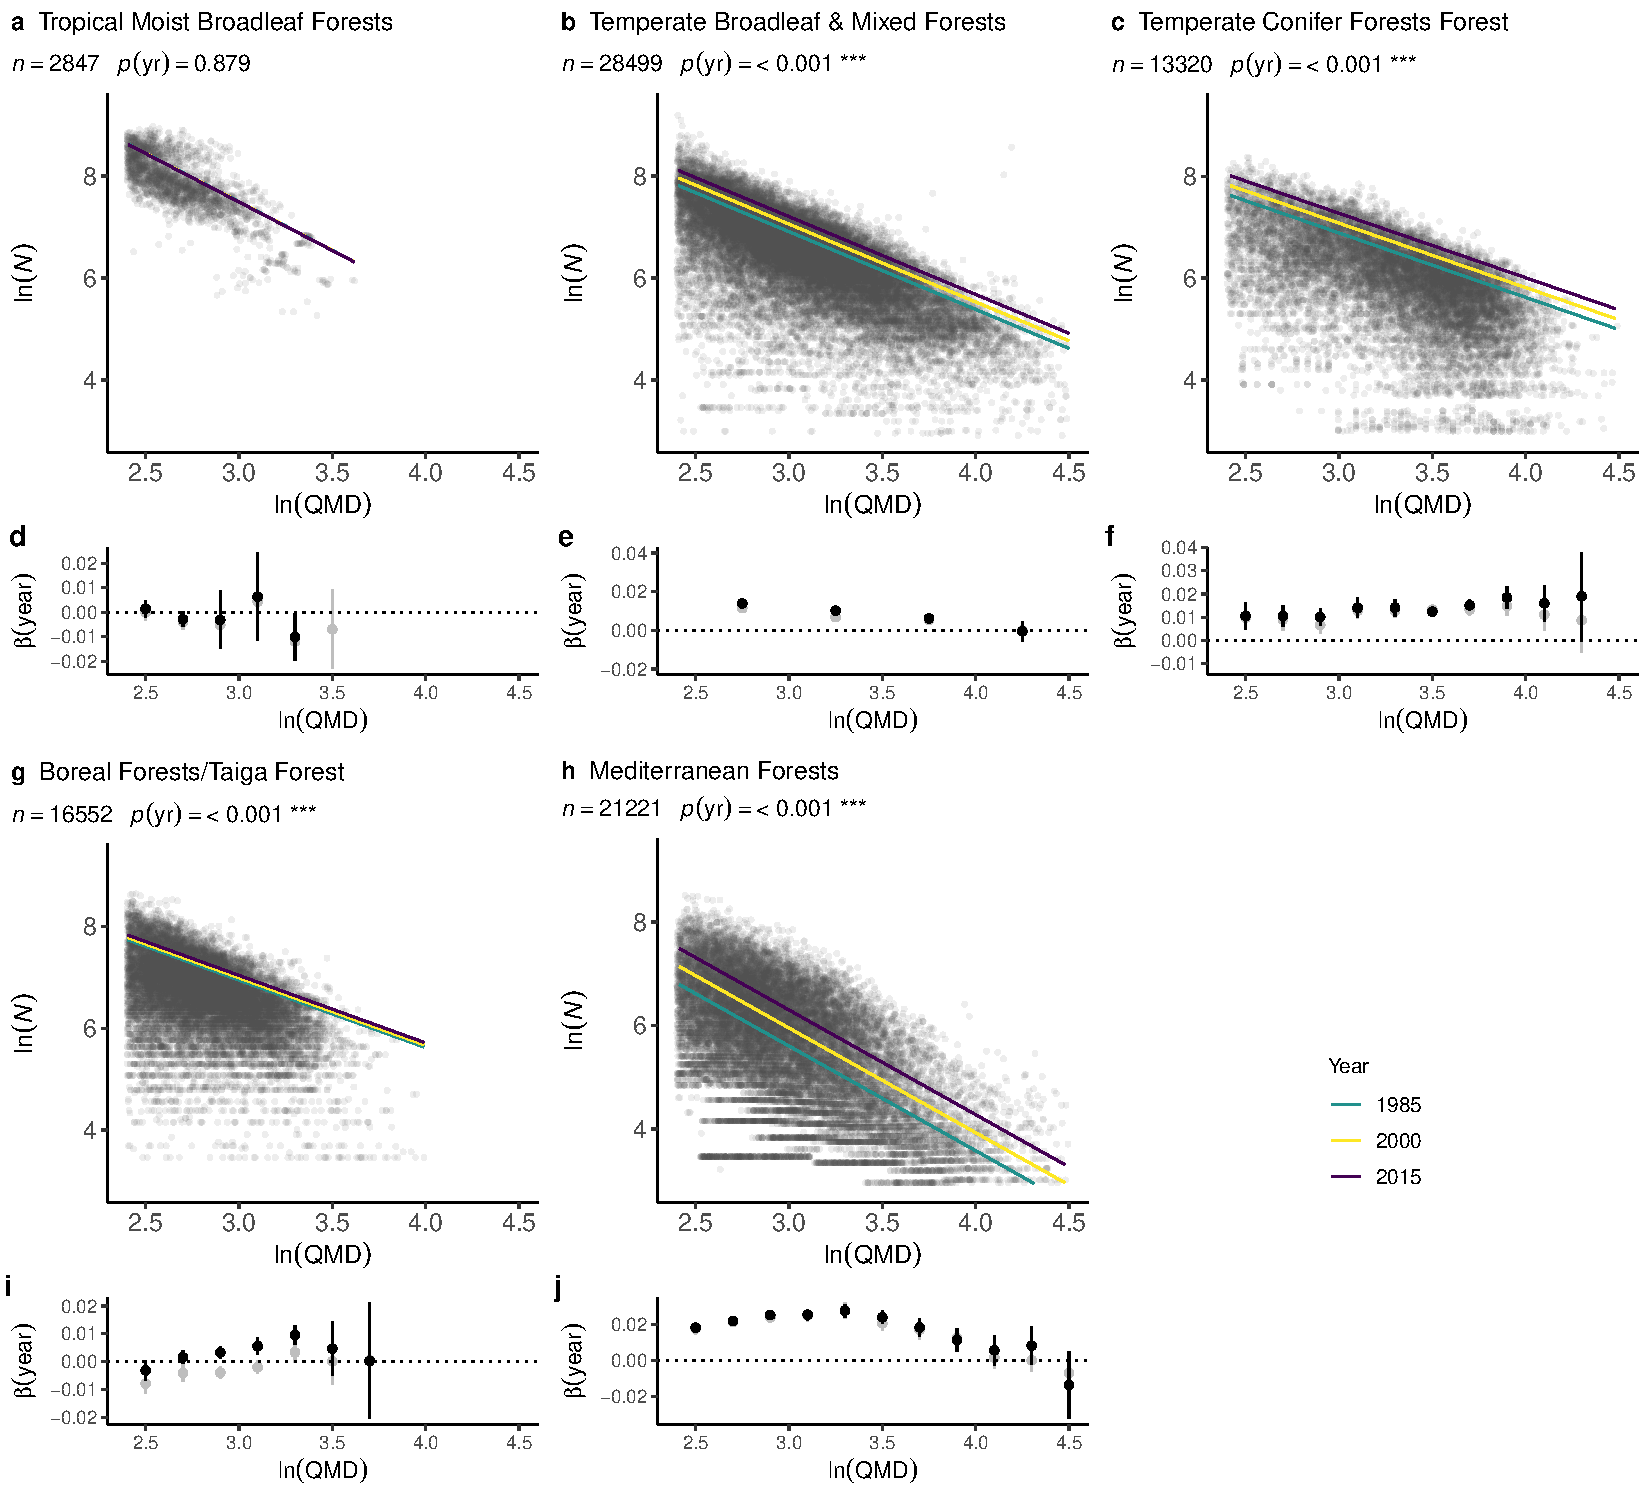
\includegraphics[width=\textwidth]{../figures/fig1_lqmm.pdf}
\caption{The caption text.}
\end{figure}

%%%%%%%%%%%%%%%%%%%%%%%%%%%%%%%%%%%%%%%%%%%%%%%%%%%%%%%%%%%%%%%%%%%%%%%%%%%
\clearpage
\bibliography{references_global_forest_thickening.bib}


\end{document}

